\documentclass[tikz,border=10pt]{standalone}
\usepackage{amsmath}
\usepackage{tikz}
\usetikzlibrary{arrows.meta, angles, quotes}
\usetikzlibrary{decorations.markings,intersections,calc}
\usetikzlibrary{shapes}
\usepackage{amssymb}
\usepackage{physics}
\usepackage{bm}
\usepackage{xcolor}
\colorlet{bordeaux}{red!70!black}
\colorlet{grey}{white!60!black}
\tikzset{omega_arrows/.style={-stealth,thick,draw=grey}}
\tikzset{L_vectors/.style={-stealth,very thick,bordeaux}}

% Parameter for the number of arrows that will be drawn
\def\NA{20}


% Parameters of the ellipsoid (h, w en d in cm)
\def\m{0.9}
\def\a{3}
\def\b{1.5}
\def\c{1.5}


\begin{document}
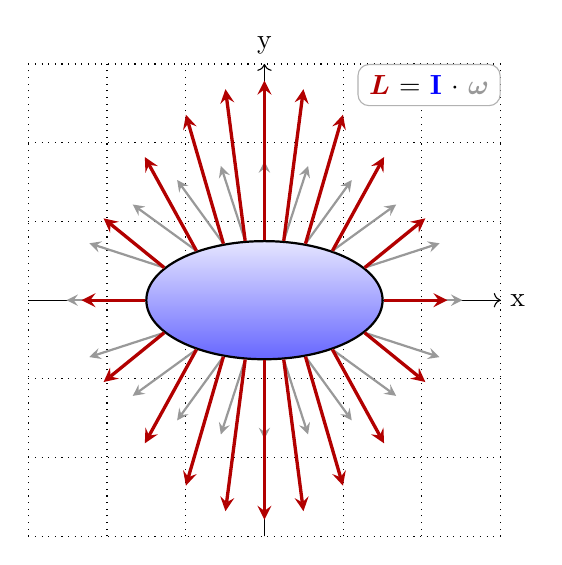
\begin{tikzpicture}

    %Define coordinate system for readability
    \draw[thin,dotted] (-3,-3) grid (3,3);
    \draw[->] (-3,0) -- (3,0) node [right] {x};
    \draw[->] (0,-3) -- (0,3) node [above] {y};

    %Draw the ellipsoid as a node:

    \node (ellipse) at (0,0)   [draw, thick, ellipse, shade,  top color=blue!10, bottom color=blue!60, minimum width= \a cm, minimum height= \b cm]{};

    % \foreach \i [evaluate={\angle=(\i-1)*360/\NA;}] in {1,...,\NA}
    %     {\draw[omega_arrows](ellipse.\angle) -- ++(\angle:1);}


    % assume that the ellipsoid has semi-axes a, b, c and mass m. The inertia tensor then becomes
    % I=[[1/5*m*(b**2+c**2),0,0],[0,1/5*m*(a**2+c**2),0],[0,0,1/5*m*(a**2+b**2)]]
    % Obviously, since this is a 2D figure, we're only interested in vectors in the XY plane. 


    % Calculate the inertia tensor components
    \pgfmathsetmacro{\Ixx}{1/5*\m*(\b^2+\c^2)}
    \pgfmathsetmacro{\Iyy}{1/5*\m*(\a^2+\c^2)}


    %For-loop over the angles
    \foreach \i [evaluate={\angle=(\i-1)*360/\NA;}] in {1,...,\NA}
      {% omega vector (length 1)
      \pgfmathsetmacro{\wx}{cos(\angle)}
      \pgfmathsetmacro{\wy}{sin(\angle)}

      % define L = I * omega
      \pgfmathsetmacro{\Lx}{\Ixx*\wx}
      \pgfmathsetmacro{\Ly}{\Iyy*\wy}

      % arrow for omega
      \draw[omega_arrows]
        (ellipse.\angle) -- ++(\angle:1);

      % arrow for L (same starting point)
      \draw[L_vectors]
        (ellipse.\angle) -- ++({\Lx},{\Ly});}

    % Legend
    \node[anchor=north east, align=left, draw=black!30, fill=white, rounded corners, inner sep=4pt]
    at (3,3) {\textcolor{bordeaux}{$\bm{L}$} = \textcolor{blue}{$\mathbf{I}$} $\cdot$ \textcolor{grey}{$\bm{\omega}$}};

\end{tikzpicture}
\end{document}